\subsubsection{First touch}
Nous allons maintenant nous concentrer sur la parallélisation du SpMV en mémoire partagée.
%
La mémoire est allouée sur un seul banc NUMA et le travail est partagée par une directive {\em \#pragma omp parallel for}.
%
Sur la machine Rostand, nous obtenons difficilement une accélération de 2,5 sur 12 coeurs en ayant 8 variables primaires (Fig.~\ref{fig:res_spmv_omp_rostand}).
%
Cette accélération descend à 1,9 en ayant 1 variable primaire, toujours sur 12 coeurs de calcul.
%
Ces résultats sont a comparer avec ceux obtenues en mémoire distribuée.
%
Nous n'obtenons que 65~\% de la puissance maximale que nous devrions avoir.
%
Le SpMV étant limité par la bande passante mémoire, l'utilisation d'un seul banc NUMA pour les accès mémoire ne nous permet pas d'exploiter toute la puissance de la machine.


%   (-_-)   %
\begin{figure}[t!]
  \centering
  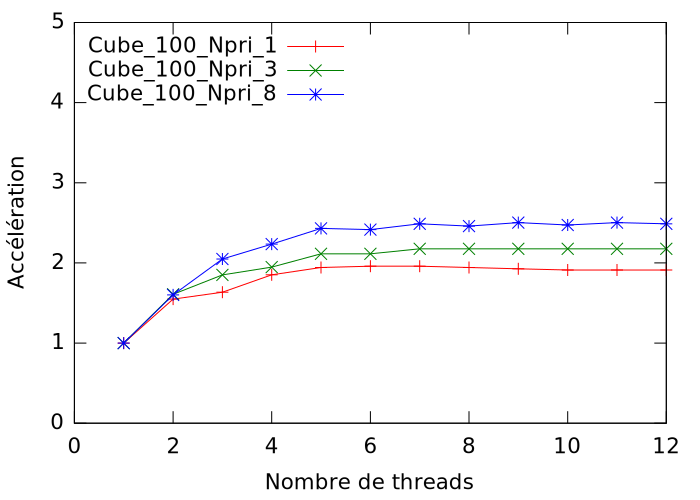
\includegraphics[width=0.7\textwidth]{res_spmv_omp}
  \caption{Accélération du produit matrice vecteur creux sur Rostand en mémoire partagée.}
  \label{fig:res_spmv_omp_rostand}
\end{figure}



Sur la machine Manumanu, ces effets sont amplifiés (Fig.~\ref{fig:res_spmv_omp_manumanu}).
%
Nous obtenons les meilleurs performances en utilisant 8 coeurs avec une accélération de 5-6.
%
Utiliser plus de 8 coeurs pour effectuer le SpMV fait perdre du temps, les données étant toute sur le premier banc NUMA, nous utilisons uniquement la bande passante de ce banc avec des latences d'accès plus ou moins longues.
%
Les résultats en mémoire distribuée sont meilleurs, en optimisant les accès mémoire de la version en mémoire partagée, nous pouvons donc espérer avoir ce même type d'accélération.


%   (-_-)   %
\begin{figure}[t!]
  \centering
  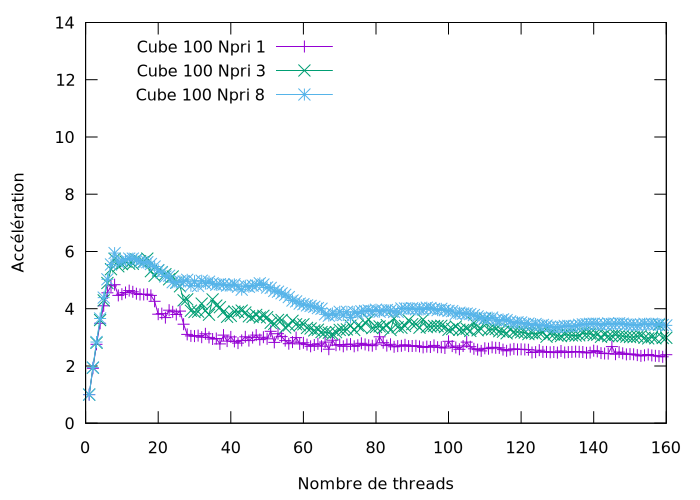
\includegraphics[width=0.7\textwidth]{res_spmv_omp_manu}
  \caption{Accélération du produit matrice vecteur creux sur Manumanu en mémoire partagée.}
  \label{fig:res_spmv_omp_manumanu}
\end{figure}
